\chapter{Theoretischer Hintergrund}
\label{chap:Theorie}
\pagestyle{plain}

Zu Beginn dieser Arbeit werde ich eine kurze Einführung in die Geschichte des Internets, und den in ihm immer größer werdenden Anteil der sozialen Medien geben. Auf letztere werde ich dann im Detail eingehen, indem ich die gängigsten Social Media Plattformen beschreibe und dann eine Übersicht der zugänglichen Plattformen gebe. Im Anschluss werde ich auf die Plattformen eingehen, die die Universität Bielefeld sich zu Nutze macht.

\section{Das Internet und die sozialen Medien}

Als Tim Berners-Lee Ende der 80er Jahre mit der Entwicklung des World Wide Web den Wissenschaftlerinnen und Wissenschaftlern des CERN in der Schweiz einen Gefallen tun, und den Austausch von Daten und Informationen innerhalb der Einrichtung für Kernforschung vereinfachen wollte \cite{w3cpeople}, hatte er sicherlich nicht das Ausmaß im Kopf, welches das Internet, so wie wir es heute kennen, annehmen, und ihm im Jahre 2004, 24 Jahre nach Beginn seiner Internet-Karriere, für seine Dienste an der globalen Entwicklung des Internets die Ritterwürde bringen sollte \cite{w3cbernerslee}. Berners-Lees Arbeit waren schon knapp zwei Jahrzehnte der Entwicklung vorangegangen, in denen über das ARPANET, welches Ende der 60er Jahre erste Gestalt annahm, am Beginn der 70er Jahre die erste Mail versendet werden konnte \cite{gillies2000web}.

Die rapide Entwicklung der Internet-Techniken begünstigt seit vielen Jahren den Informationsaustausch und die Möglichkeit zur individuellen und Gruppen-Kommunikation und vereinfacht diese stets weiter. So sind die Dienste des Internets schon lange nicht mehr ein Privileg von Forschungseinrichtungen wie dem CERN, Universitäten, oder militärischen Einrichtungen. Über 50 Prozent der Erdpopulation hat bereits regelmäßigen Internetzugang, wie eine statista-Studie von Juli diesen Jahres zeigt \cite{statista2018digpop}. Eine solch hohe Zahl ist auch der Entwicklung der sozialen Medien zu verdanken, wie man den Nutzungsstatistiken der großen Social Media Plattformen entnehmen kann, auf die später in diesem Kapitel noch eingegangen wird.

Die Nutzung des Internets, und den in ihrer Popularität immer weiter steigenden Social Media Plattformen, die "[...] einen neuartigen Raum zwischen massenmedialen und der interpersonalen Kommunikation schaffen und einnehmen"\  \cite{schmidt2018einstieg}, ist aus dem Alltag der meisten Menschen überhaupt nicht mehr wegzudenken. Doch was gehört zu diesen Social Media Plattformen dazu? Warum ist eine Internetnutzung ohne Social Media Plattformen heutzutage nicht mehr denkbar? Im Folgenden möchte ich eine Übersicht über bekannte Social Media Plattformen geben, um diesen Fragen nachzugehen.

\subsection{Social Media Plattformen}

\subsubsection{Facebook}

Die wohl bekannteste und meist genutzte Social Media Plattform ist Facebook \faFacebook. Mit täglich ca. 1,4 Milliarden Nutzerinnen und Nutzern \cite{facebookfinancials} nutzten laut des eigenen Firmenreports im Dezember 2017 jeden Tag ein knappes Fünftel der gesamten Menschheit, also ein knappes Drittel der aktiven Internetnutzer, Facebook. Facebook kombiniert viele Gesichtspunkte der sozialen Kommunikation und Interaktion in einer Oberfläche, was eine vielfältige Nutzung ermöglicht. Angefangen mit klassischer Eins-zu-eins-Kommunikation im privaten Chat, über private Gruppenkommunikation bis hin zu öffentlichen Diskussionsmöglichkeiten in wiederum geschlossenen oder öffentlichen Interessensgemeinschaften, bietet Facebook seinen Nutzerinnen und Nutzern das gesamte Spektrum der sozialen Kommunikation. Über die direkte Kommunikation hinaus, ist die indirekte Kommunikation zur Außenwelt --ob einer eingeschränkt privaten, oder aber auch der gesamten, öffentlich zugänglichen-- ein großer Teil der Social Media Plattform und gleichzeitig auch der Bildung von persönlichen Öffentlichkeiten, einem "[...] Geflecht von online zugänglichen kommunikativen Äußerungen zu Themen von vorwiegend persönlicher Relevanz [...]"\ \cite{schmidt2009netz}.

Auf Facebook ist es der Nutzerin und dem Nutzer möglich, sowohl Text- als auch Bild- und Video-Beiträge zu erstellen, oder aber auf im Internet schon vorhandene Information zu verlinken. Dabei kann die sogenannte Timeline, also die chronologische Gesamtheit der Beiträge einer Nutzerin oder eines Nutzers, zur Informationsweitergabe, zur Dokumentation eigenen Wissens oder eigener Erlebnisse, oder aber auch zum Aufbau oder zum Erhalt von Beziehungen dienen.

Zusätzlich zu dieser Produzenten-Funktion kommt bei den meisten Social Media Plattformen --auch bei Facebook-- die Funktion des Rezipienten hinzu. Die Nutzerin und der Nutzer der Plattform Facebook kann nicht nur eigene Inhalte teilen sondern gibt mit der Veröffentlichung eigener Informationen und Beiträge auch anderen Nutzerinnen und Nutzern die Möglichkeit, auf Beiträge zu reagieren und/oder zu kommentieren und auch die Beiträge weiter auf der eigenen Timeline oder in anderen Gruppen/Interessensgemeinschaften zu teilen.

\subsubsection{Weblogs}

Weblogs, im weiteren Verlauf verkürzt Blogs, sind eine digitale Form des Tagebuchs. Der Begriff setzt sich aus den Teilen \textit{Web} und \textit{Log(buch)} zusammen. Der Unterschied zwischen einer Social Media Plattform wie Facebook, und dem klassischen Blog, ist die Funktion der/des Blogführenden. Diese/r nimmt in erster Linie nur die Rolle des Produzenten ein, da es sich beim klassischen Blog um die Herausgabe von Informationen und Wissen von einer stärker als bei anderen Social Media Plattformen eingeschränkten Personengruppe handelt. So werden einige der bekanntesten Blogs von Einzelpersonen geführt\footnote{Beispiele im deutschsprachigen Raum:\\Fefes Blog, \url{https://blog.fefe.de/}; Technikfaultier, \url{https://www.technikfaultier.com}}; einige andere wiederum von kleinen Personengruppen. Auch Firmen und Institutionen machen sich mittlerweile Blogsysteme zu nutze, um in klassischer Zeitungsmanier regelmäßig Informationen zu verbreiten.

In den meisten Blogsystemen sind mittlerweile Kommentarfunktionen eingebaut, die mehr oder minder häufig von den Betreibenden auch genutzt werden. Da es sich hierbei jedoch nicht unbedingt um einen Kernbaustein des Systems handelt, ist dieser Funktions-Unterschied zu anderen Social Media Plattformen entscheidend.

Zu den am häufigsten genutzten Blog-Plattformen gehören WordPress \faWordpress, Googles Blogger und Medium \faMedium.

\subsubsection{Twitter}

Twitter \faTwitter\ ist der populärste Vertreter der Blog-Unterkategorie Mikroblog. Ein besonderes Merkmal der Plattform ist, dass Beiträge in Ihrer Länge stark limitiert sind. Angefangen bei nur 140 Zeichen, ist die Begrenzung mittlerweile auf 280 Zeichen angehoben worden. Dennoch bleibt Twitter eine der wenigen populären Mikroblog-Plattformen.

Ein Tweet, also ein Beitrag auf Twitter, kann innerhalb der 280 Zeichen normalen Text, aber auch Bilder und Kurzvideos und Links zu anderen Webseiten oder Medien darstellen. Die Besonderheit dabei ist die Möglichkeit zum einen, einen Tweet mit Schlagworten, sogenannten \textit{Hashtags} zu versehen, indem dem gewünschten Schlagwort ein \# vorangestellt wird, und zum anderen die Möglichkeit, andere Nutzerinnen und Nutzer der Plattform direkt zu adressieren, indem dem Nutzernamen der zu kontaktierenden Person ein @ vorangestellt wird. Der Tweet \textit{"@wohfab recherchiert zum Thema \#socialmedia."} würde also den Autor dieser Abschlussarbeit direkt adressieren und ihn über den Tweet benachrichtigen, und jeder Nutzerin und jedem Nutzer die Möglichkeit geben, nach dem Schlagwort \textit{\#socialmedia} zu suchen, und andere Beiträge mit gleichem Schlagwort zu finden und zu lesen. Beide sogenannten Tags, also sowohl die Hashtags als auch die Namenstags, werden bei Twitter automatisch zu anklickbaren Links.

Die Tweets können dann von anderen Nutzerinnen und Nutzern mit einem Herz markiert, kommentiert, und in der eigenen Twitter-Historie geteilt werden. Letzteren Vorgang wird innerhalb der Plattform als Retweeten -- also \textit{nochmal Tweeten} -- bezeichnet.

\subsubsection{Instagram}

Als Tochterfirma von Facebook \cite{instagramtou}, hat sich Instagram \faInstagram\ auf die Nutzung auf mobilen Endgeräten, und auf visuelle Medien spezialisiert. Angefangen mit Bildern, können mittlerweile auch Videos in normalen Beiträgen und sogenannten Stories geteilt werden. Letztere sind in einem zeitlich begrenzten Rahmen sichtbar und werden danach für die Öffentlichkeit unzugänglich gemacht. In Abgrenzung zu einem klassischen Blog, sind Beiträge auf Instagram --insbesondere die Story-Beiträge-- also eher kurzlebig.

Wie Twitter --und mittlerweile auch Facebook-- setzt Instagram stark auf die Nutzung von Hash- und Namenstags zur Kategorisierung und Adressierung von Beiträgen. Gegenüber Twitter hat Instagram den Vorteil, dass die Beiträge in Ihrer Länge nicht stark limitiert sind. Ein Instagram-Beitrag kann also sehr umfangreich kommentiert und zusätzlich mit einer großen Menge an Schlagworten ausgezeichnet werden. Besonders um über den eigenen Nutzerkreis hinaus Bekanntheit zu erlangen, werden für Instagram-Beiträge eine Vielzahl an Schlagworten genutzt, die sich auch wie die Timelines von Nutzerinnen und Nutzern abonnieren lassen.

\subsubsection{Snapchat}

Eine ebenfalls auf Bild- und Videomaterial spezialisierte Social Media Plattform ist Snapchat \faSnapchat. In Abgrenzung zu Instagram basiert Snapchat vollständig auf der Kurzlebigkeit seiner Beiträge, die nach geringem Zeitfenster grundsätzlich der Öffentlichkeit unzugänglich gemacht werden. Trotz der sehr speziellen Art dieser Plattform, begeistern sich jedoch täglich mehr Nutzerinnen und Nutzer an Snapchat.

\subsubsection{Karriere-Plattformen - LinkedIn und XING}

Mit LinkedIn \faLinkedin\ und XING \faXing\ sind wir mittlerweile bei den eher untypischen Social Media Plattformen angekommen. Diese beiden Plattformen können der Kategorie Karriere-Plattform zugeordnet werden. Sie dienen der Vernetzung innerhalb der Berufswelt. XING beschränkt sich dabei sehr auf den deutschsprachigen Raum; LinkedIn wird international genutzt. Ansonsten unterscheiden sich die beiden Plattformen nur in wenigen Details.

Auf solchen Karriere-Plattformen lässt sich ein Profil anlegen, auf dem der schulische und berufliche Werdegang, abgeschlossene Schulungen und erhaltene Zertifikate, besonderes Wissen und besondere Fähigkeiten und Karriere- und Forschungsinteressen mit der Öffentlichkeit oder bestimmten Personenkreisen geteilt werden können. 

\subsubsection{WhatsApp, Telegram und co.}

Auch sogenannte Instant Messaging Dienste, deren Kernfunktion die Direktkommunikation zwischen zwei Nutzerinnen/Nutzern ist, zählen zu den Social Media Plattformen. SMS und MMS aus früheren Jahren sind in unseren Breitengraden mittlerweile von Diensten wie WhatsApp \faWhatsapp, Telegram und co. abgelöst worden. Der Messaging Dienst von Facebook gehört ebenfalls zu diesen Instant Messaging Diensten. Lange Zeit war dieser an einen Facebook-Account geknüpft. Inzwischen kann man den Facebook Messenger mit einer Telefonnummer und unabhängig von einem Facebook-Account nutzen. iMessages \faApple\ ist ein Apple-Exklusiver Instant Messaging Dienst, der im Apple-Ecosystem große Beliebtheit erlangt hat; dessen größter Nachteil jedoch die System-Exklusivität ist. WhatsApp hat laut eigener Angabe im firmenblog über eine Milliarde aktive Nutzer täglich \cite{whatsappblog} und ist somit der meistgenutzte Instant Messaging Dienst weltweit.

\subsubsection{Audio- und Video-Telefonie mit Skype und Discord}

So wie Skype \faSkype, gehört auch Discord zu den Audio- und Video-Chat-Plattformen. Skype gehörte lange zur Standardplattform für Video-Telefonie und wird auch heutzutage im Enterprise-Bereich noch häufig genutzt. Discord kam vor nicht allzu langer Zeit auf diesem Markt hinzu und startete als Kommunikationsplattform für Videospielende. Die Simplizität, der Funktionsumfang der Applikationen und sowohl die Audio- als auch die Video-Qualität der Plattform haben Skype jedoch in vielen Fällen überholt und für viele Nutzerinnen und Nutzer ersetzt.

Als weitere Audio-Kommunikations-Plattformen sind noch TeamSpeak und Mumble zu nennen, die ebenfalls im Videospiel-Klientel ihre Ursprünge haben; jedoch wie Skype auch in vielen Fällen durch Discord abgelöst wurden.

\subsubsection{Wikis als moderne Variante des Forums}

Ebenfalls eher untypische Social Media Plattformen sind sogenannte Wikis. Sammlungen von Wissen, sogenannte Knowledge Bases, wie die Online-Enzyklopädie Wikipedia, setzen auf die Zusammenarbeit der Nutzerinnen und Nutzer, um die Gesamtheit des Weltwissens zu archivieren. Die Wikipedia \faWikipediaW\ ist mit Sicherheit die größte öffentlich zugängliche Knowledge Base und bekommt nach eigenen Angaben alleine auf der deutschen Variante im Durchschnitt über 32 Millionen Aufrufe pro Tag \cite{wikipediastatistik}. Neben der Wikipedia gibt es eine schier unendliche Masse an Wikis, die sich mit zum Teil sehr spezifischen, eingeschränkten Themenbereichen auseinandersetzen und häufig eine moderne Variante eines Forums darstellen, was in den Anfängen der Social Media Plattformen eine sehr übliche Art der Wissenserhaltung und der sozialen Kommunikation war.

\subsubsection{Reddit, die Startseite des Internets}

Ebenfalls Ähnlichkeiten zum klassischen Forum, weist Reddit \faReddit\ auf. Reddit kann als Meta-Forum bezeichnet werden. Es ist in mittlerweile ca. 1,2 Millionen Unter-Foren, sogenannte Subreddits aufgeteilt \cite{redditmetrics}, die sich jeweils unterschiedlichen Thematiken widmen. Diese Subreddits reichen von Nachrichten-Seiten, über Fan-Seiten für Film \& Fernsehen, bis hin zu Spaß-Seiten, die dem reinen Vergnügen dienen.

\subsubsection{Weitere Plattformen}

Neben den oben genannten Plattformen existiert eine große Menge an weiteren Plattformen, von denen ich einige bekannte Vertreter zumindest erwähnen und kategorisieren möchte.

\textbf{Video} -- YouTube \faYoutube\ und Vimeo \faVimeo\ gehören beispielsweise zu den Video-Plattformen. Die Kernfunktionalität der Plattformen ist das Veröffentlichen von fertigen Videos. Im Gegensatz dazu, setzt zum Beispiel Twitch auf die Funktionalität des Streamings. Videos werden also live übertragen, statt sie zu bearbeiten und zu schneiden, um sie dann im fertigen Format hochzuladen. Twitch ist sehr beliebt im Gaming-Bereich.

\textbf{Foto} -- Flickr \faFlickr\ , Behance \faBehance\ , 500px \faicon{500px}, Deviantart \faDeviantart\ sind Vertreter der Foto-Plattformen. Behance hat zusätzlich zum Teilen selbst erstellter Fotos einen besonderen Fokus auf Grafikdesign und die Monetarisierung desselben. Deviantart ist eine Indie-Grafiker-Plattform, die zu großen Teilen für sogenannte Fanarts verwendet wird.

\textbf{Audio} -- Die wohl bekannteste soziale Audio-Plattform ist Soundcloud \faSoundcloud. Nicht nur Künstlerinnen und Künstler können hier Ihre Werke veröffentlichen und mit ihren Fans über Kommentare und Reaktionen auf die hochgeladenen Stücke in Kontakt kommen. Soundcloud bietet eine Plattform für jegliche Art von Audiomaterial.

\textbf{Chat} -- IRC, Internet Relay Chat, wird oft mit Computerspezialistinnen und -spezialisten, meist auch mit Hackern in Verbindung gebracht. Das rein textbasierte Chatsystem läuft ohne viel Aufwand und ohne viel Ressourcen auf nahezu jedem Server und bietet somit für die Kommunikation über reinen Text eine praktische Plattform. IRC ist organisiert in Server und innerhalb dieser in sogenannte Channels, die sich zur besseren Übersicht in bestimmte Themenbereiche einteilen.

\subsubsection{Übersicht}

Alleine die Zusammenfassungen der oben genannten, bekanntesten Social Media Plattformen ist sehr umfangreich, was einen Hinweis auf die Masse an Plattformen geben kann, die in ständiger Benutzung sind und sich täglich weiterentwickeln.

\begin{figure}[h]
    \centering
    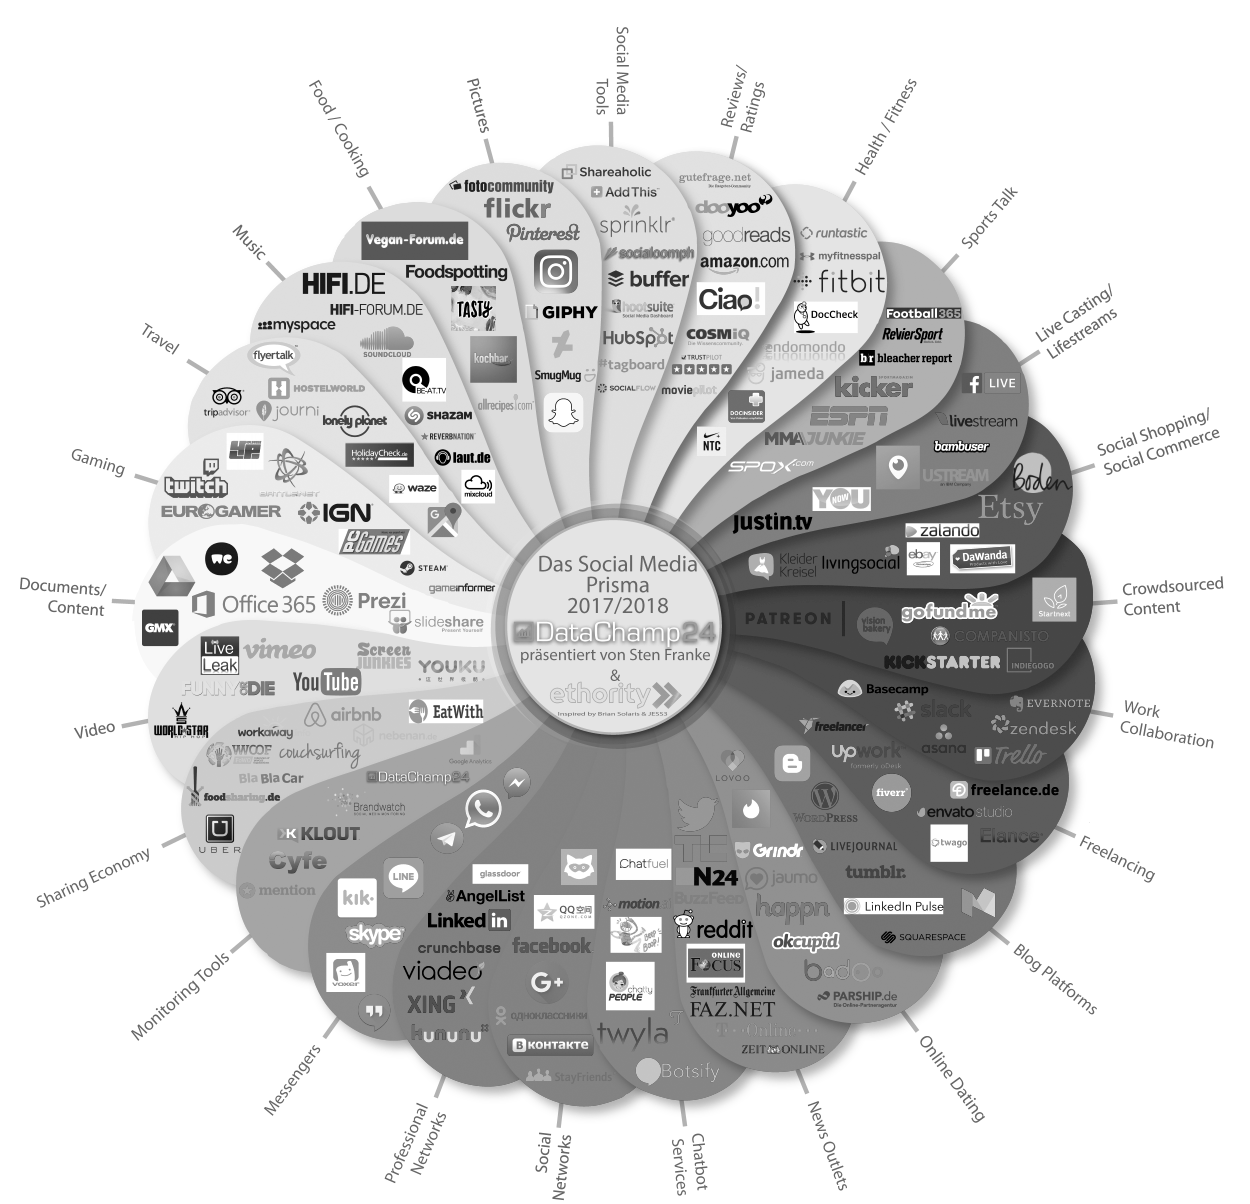
\includegraphics[width=\textwidth]{img/ethority-smp-bw.png}
    \caption{Schaubild zur Übersicht von Social Media Tools aus dem Jahresbericht der Digitalagentur \textit{ethority}. \\ \cite{ethorityprisma2018}}
    \label{fig:socialmediatoolsethority}
\end{figure}

Der Digital-Blog \textit{ethority} stellt regelmäßig ein Schaubild über die meistgenutzten Social Media Plattformen her und veröffentlicht dieses. Der Vollständigkeit halber möchte ich dieses in Abbildung \ref{fig:socialmediatoolsethority} auch zeigen, um die Übersicht zu komplettieren.



Dieses Schaubild verdeutlicht noch einmal die Vielfalt und Masse der Social Media Plattformen, die auf täglicher Basis von bis zu über einer Milliarde Menschen genutzt werden. Wo Privatpersonen, gerade im Hinblick auf die eigene Privatsphäre, sich im Normalfall einer geringeren Anzahl verschiedener Social Media Plattformen bedienen; auch, weil das intendierte Publikum auf vielen Plattformen meist ein limitierter Kreis an Bekannten ist, müssen Unternehmen und Institutionen, die mit Hilfe der Social Media Plattformen ihren Einfluss und ihre Reichweite vergrößern möchten, auf eine Vielzahl von unterschiedlichen Plattformen zurückgreifen.

\section{Die Social Media Kommunikation der Universität Bielefeld}

Die Universität Bielefeld --hier als Beispiel einer Institution-- nutzt ebenfalls diverse Social Media Plattform zur Verbreitung von Inhalten. Auf der Webseite der Universität lassen sich vier der genutzten Plattformen direkt über Icons erreichen.

\begin{figure}[h]
    \centering
    
\includegraphics[width=\textwidth]{img/uni-smp-bw.png}
    \caption{Webseite der Universität Bielefeld mit Social Media Menüs im Header und Footer (mit Rechtecken umrandet). Zur besseren Übersicht, wurde der inhaltliche Teil der Webseite entfernt.}
    \label{fig:socialmediatoolsuni}
\end{figure}

Die mehrfache Auflistung der genutzten Plattformen ist im Online Marketing üblich, um bei Webseiten mit längeren Inhalten an möglichst jeder Stelle, auf der sich die Nutzerin/der Nutzer befindet, auf das Angebot verlinken zu können.

In dem sogenannten Social Media Menü werden hier die Angebote Facebook, Twitter, YouTube und Instagram verlinkt. Eine weitere Social Media Plattform, die sich die Universität zu nutze macht, ist ein Blog, der über die Webseite \texttt{\href{http://ekvv.uni-bielefeld.de/blog/uninews/}{ekvv.uni-bielefeld.de/blog/uninews}} erreichbar ist. Eine Besonderheit des Blogs ist, dass sich dieser in verschiedene Unter-Blogs einteilt, über die zum Beispiel auch einzelne Fakultäten, universitäre Einrichtungen oder sogar Einzelpersonen verfügen können. Gegenüber den im Consumer-Bereich häufig genutzten, oben schon angesprochenen, Blogsystemen, wie WordPress oder Blogger, bedienen sich die vom Bielefelder Informationssystem (BIS) verwalteten Blogs dem Blog-System \textit{Apache Blog Roller}.

Ebenfalls für Einrichtungen und Mitarbeiterinnen und Mitarbeiter der Universität zugänglich, ist ein Wiki-System, welches auf der Software \textit{JAMwiki} basiert. Da die Universität als Gesamtinstitution davon jedoch keinen Gebrauch macht, werde ich dieses im weiteren Verlauf außer Acht lassen.

Um aufzeigen zu können, in welchem Maße die verschiedenen Plattformen von den Benutzern genutzt werden, zeige ich die aktuellen Zahlen der Follower aus September 2018 auf. Dabei handelt es sich bei Instagram und Twitter um die Zahlen der Follower, bei YouTube um die Abonnenten des Kanals, und bei Facebook um die Nutzerinnen und Nutzer, die die Facebook-Fanpage der Universität Bielefeld mit einem Like markiert haben.


\begin{figure}[h]    
    \centering
    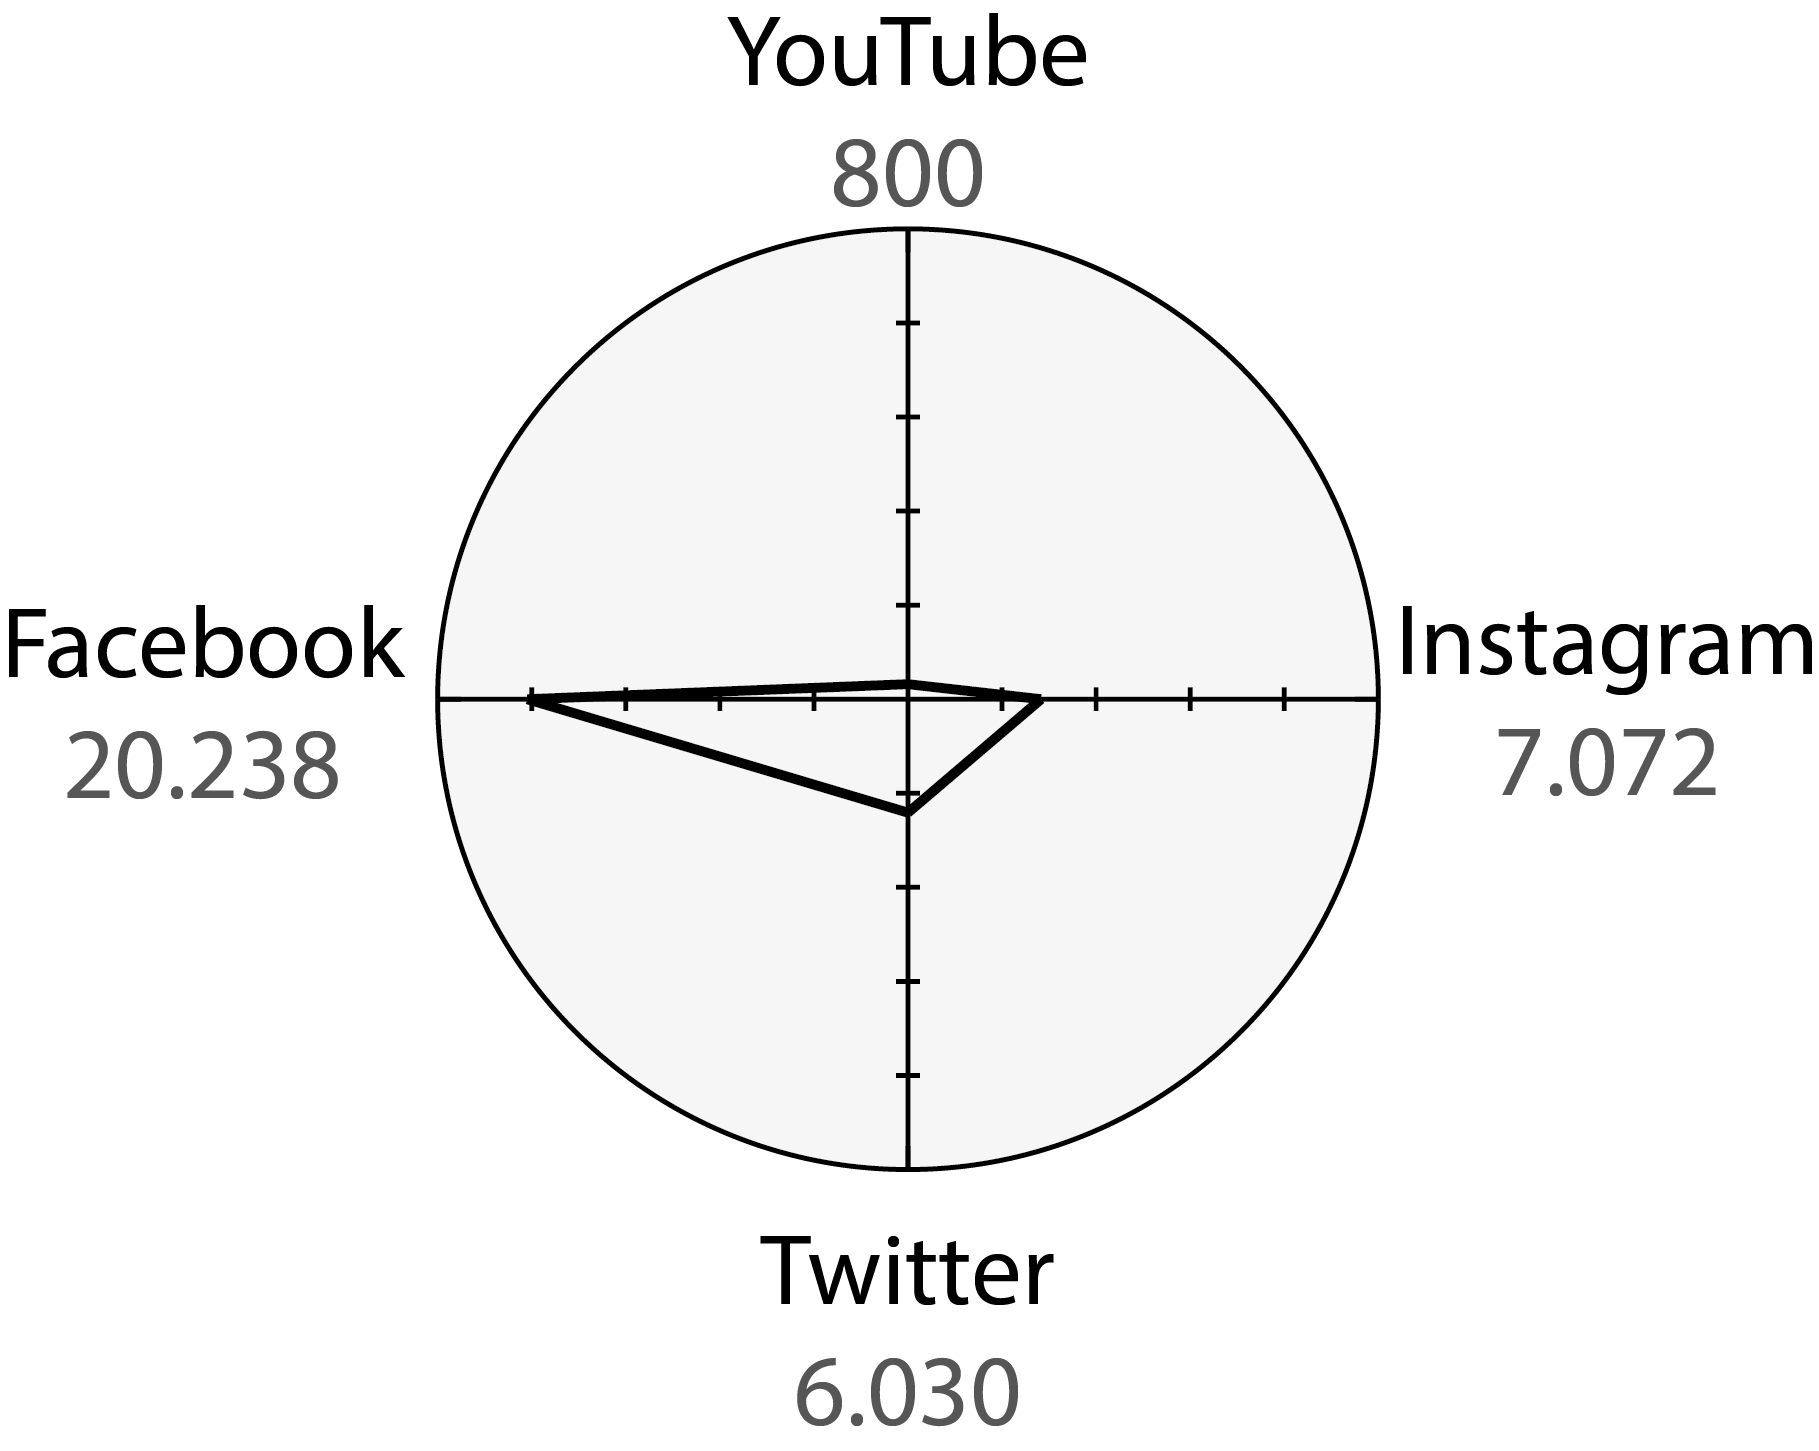
\includegraphics[width=.8\textwidth]{img/posts/follower_gesamt.png}
    \caption{Follower der Social Media Plattformen, die von der Universität Bielefeld genutzt werden in einem Radar-Graphen dargestellt. Ein deutlicher Überhang der Plattformen Facebook, Twitter und Instagram gegenüber dem YouTube-Kanal ist zu erkennen (Stand: September 2018).}
    \label{fig:follower}
\end{figure}

\begin{table}[h]
    \centering
        \caption{Prozentuale Verteilung der Follower der von der Universität Bielefeld genutzten Social Media Plattformen.}
        \begin{tabular}{*{5}{l}}
        Facebook & Universitäts-Blog & Instagram & YouTube & Twitter \\
        \hline
        59,28 \% & nicht messbar & 20,71 \% & 2,34 \% & 17,66 \%
        \end{tabular}
    \label{tab:followerprozent}
\end{table}

Insgesamt 34.140 Follower hat die Universität Bielefeld auf ihren Social Media Plattformen. Davon nutzen mit knapp 60 \% Facebook die meisten, und mit nur knapp 2,3 \% YouTube die wenigsten Follower. Twitter nimmt knapp 18 \%, und Instagram knapp 21 \% der Gesamtfollower ein. Dabei ist, wie oben angegeben, zu beachten, dass die Zahl der Blog-Follower nicht messbar ist, da dieser unter anderem auch per RSS-Feed zugänglich ist, welcher die Besucherzahlen nicht preisgibt.

\section{Forschung -- Jan-Hinrik Schmidt}
\label{sec:aktuelleforschung}

Das folgende Kapitel dient der Übersicht des aktuellen Standes der Social Media Forschung. Ausgehend von Jan-Hinrik Schmidts \textit{"Was ist neu am Social Web?"}, werde ich in diesem Kapitel im Allgemeinen auf Schmidts Forschung im Bereich der sozialen Medien eingehen und seine Begriffswahl erläutern. Danach widme ich mich im Speziellen dem von ihm geprägten Kommunikations-Modell, das die Begrifflichkeit dreier Leistungen definiert, die durch Anwendungen im Social Web unterstützt werden \cite{schmidt2008neu}.

\subsection{Social Media wird zu \textit{Social Web}}

Die Social Media Kommunikation lässt sich dem Namen entsprechend relativ einfach innerhalb der Linguistik in den Bereich der Kommunikationswissenschaft einordnen. Als Kommunikationswissenschaftler mit Wurzeln in der Soziologie kritisiert Jan-Hinrik Schmidt den von O'Reilly (2004) geprägten Begriff des Web 2.0 und postuliert, jene Bezeichnung mit dem Begriff Social Web zu ersetzen. Die Bezeichnung 2.0, die sich der Notation der üblichen Versions-Nummerierung in Computer-Anwendungen bedient, vermittle grundlegende und schrittartige Veränderungen. Die zu beobachtenden Veränderungen verlaufen jedoch fließend, weshalb Schmidt die Versions-Nummerierung für ungünstig hält und einen Gegenvorschlag liefert.

Der Begriff \textit{Social Web} soll die Wichtigkeit der sozialen Aspekte in den Vordergrund stellen, da in der Zeit des Produsers\footnote{Ein Produser nimmt in einem einzigen Netzwerk sowohl die übliche Rolle des Rezipienten als auch die eher unüblichere Rolle des Produzenten gleichzeitig ein.} die Internet-Kommunikation weit über die Kommunikation von Mensch zu Maschine hinausgeht und immer mehr Nutzerinnen und Nutzer zu solchen Produsern werden, statt die sozialen Medien einzig zur Rezeption zu nutzen. Das Weglassen der Versions-Nummerierung soll den stetigen Wandel der sozialen Medien verdeutlichen. Im weiteren Verlauf dieser Arbeit möchte ich mich an dieser Begrifflichkeit orientieren.

"Wie jede andere Form des sozialen Handelns auch ist die Nutzung des Social Web durch die Dualität von Struktur und Handeln gekennzeichnet", so Schmidt. Diese Dualität, die Schmidt mit \cite{giddens1988konstitution} zitiert kann ebenfalls auf die Analyse von Social Web Kommunikation angewandt werden (vgl. \cite{schmidt2006social} \& \cite{schmidt2006weblogs}). Dabei ist, um das Handeln und die sozialen Strukturen zu verbinden, das Konzept der Nutzungspraxis von entscheidender Bedeutung.

Schmidt nennt dieses Konzept die Manifestation gerahmter Nutzungsabsichten, und erläutert die erwähnte Rahmung im Detail. Zu ihr gehören unterschiedlich explizite und sanktionierbare Verwendungsregeln; von selbst erstellten Verhaltenskodizes -- in zum Beispiel privaten Chat-Gruppen -- über Geschäfts- und Nutzungsbedingungen von Social Web Plattformen, bis hin zu juristischen Regelungen, wie sie beispielsweise über das Inkrafttreten der EU Datenschutzgrundverordnung (EU DSGVO) \cite{eurlex2016} im Mai diesen Jahres großes Aufsehen erregt haben. Neben diesen Verwendungsregeln spielen zwei weitere strukturelle Dimensionen eine Rolle: Zum einen der Code, der die softwaretechnischen Grundlagen einer Social Web Anwendung festlegt, indem er die Möglichkeiten, die eine Anwendung der Nutzerin/dem Nutzer bietet, überhaupt erst erschafft; jedoch gleichzeitig auch einschränkt. (Für letztere Funktionsweise des Codes ist die Zeichen-Limitierung von Beiträgen auf Twitter ein hervorragendes Beispiel.) Zum anderen die Relationen, die im hypertextuellen Zusammenhang die Verknüpfungen von Stellen innerhalb eines Dokuments -- sogenannte \textit{intra}textuelle Hyperlinks -- oder aber auch die Verknüpfungen von verschiedenen Dokumenten miteinander -- sogenannte \textit{inter}textuelle Hyperlinks -- darstellen.

Von der Beschreibung der Nutzungspraxis kommt Schmidt zu den Leistungen, die das Social Web unterstützt. Diese Leistungen stellen den Kern der Forschung dar, auf die diese Arbeit aufbaut, und auf die ich im folgenden Kapitel eingehen werde.

\subsection{Modell der Social Web Kommunikation}
\label{sec:jhsforschung}

Drei Funktionen werden nach Schmidt von den Anwendungen im Social Web unterstützt. Hierbei handelt es sich um Formen des Managements der persönlichen Öffentlichkeit einer Nutzerin/eines Nutzers. 

Die erste Funktion ist das \textit{Identitätsmanagement}. Innerhalb des Identitätsmanagements macht die Nutzerin/der Nutzer spezifische Teile der eigenen Person publik, was zur Entwicklung der eigenen persönlichen Öffentlichkeit beiträgt. Die von Schmidt angesprochene Leistung, die das Identitätsmanagement erbringen kann, ist das selektive Präsentieren der eigenen Person. Die Nutzerin/Der Nutzer kann Aspekte der eigenen Person vor der Veröffentlichung filtern, und bleibt somit gewissermaßen in Kontrolle. Unter prototypische Anwendungen, die das Identitätsmanagement unterstützt, fallen beispielsweise Blogs, Pod- und Videocasts, Nutzerprofile auf Social Web Plattformen und Video-Plattformen, wie YouTube und Vimeo. Über diese Anwendungen können bestimmte Aspekte der eigenen Person, wie Meinungen, Interessen, Weltanschauungen, Wissen, etc. präsentiert werden.

Die zweite Funktion ist das \textit{Beziehungsmanagement}. Hierbei werden die Anwendungen des Social Web dazu genutzt noch nicht existente Beziehungen zu knüpfen und vorhandene Beziehungen auszubauen oder zu verändern. Das Netzwerken, sowohl privat über Plattformen wie Facebook als auch auf professioneller, beruflicher Ebene, beispielsweise über LinkedIn und XING, ist in Schmidts Modell die soziale Form der Hyperlinks. Diese stellen, wie oben bereits angesprochen, intra- oder intertextuelle Verknüpfungen her. Übertragen auf die persönliche Öffentlichkeit, stellen diese also interpersonelle Beziehungen her, indem man zum Beispiel über Facebook eine andere Nutzerin/einen anderen Nutzer als Freundin/Freund hinzufügt.

Die dritte Funktion der Social Web Anwendungen ist das \textit{Informationsmanagement}. Bei diesem geht es sowohl um die Produktion als auch die Rezeption von Informationen. Prototypische Anwendungen sind zum Beispiel Wikis. Aber auch kollaborative Wissensplattformen, wie diverse Reddit Unterforen, oder die von Y Combinator erstellte Plattform \textit{Hacker News}, die für Programmierer  -- und auch für die Open Source Bewegung -- Technik-Nachrichten aggregiert, zählen zu den prototypischen Anwendungen, die die Funktion des Informationsmanagements unterstützen. Die vom Informationsmanagement erbrachten Leistungen umfassen neben dem Auffinden und der Rezeption von Informationen auch deren Verwaltung. Letztere Leistung ist besonders in der Open Source Bewegung und in der Gruppe der SystemadministratorInnen häufig durch sogenannte \textit{Personal Knowledge Bases} -- also private Wissenssammlungen -- abgedeckt. Eine solche Knowledge Base kann ebenfalls ein privat angelegtes Wiki sein, dass dann einzig zur Verwaltung eigenen Wissens dient.

%\newpage
\section{Forschungsfragen und Hypothesen}
\label{sec:hypothesen}

In diesem Abschnitt werde ich aus den vorangegangenen Kapiteln Forschungsfragen herleiten und diese zu Hypothesen formen. Dabei gehe ich sowohl auf die Nutzerinnen- und Nutzerseite der Social Web Plattformen als auch auf die in \ref{sec:aktuelleforschung} erarbeiteten Forschungsgrundlagen ein, um die Hypothesen zu begründen.

Wie in \ref{sec:jhsforschung} deutlich wurde, ist das Modell nach Jan-Hinrik Schmidt ein auf die Einzelperson zugeschnittenes Modell. Wo einige Aspekte des Social Web, wie zum Beispiel der der Social Web Anwendungen zugrunde liegende Code (vgl. \cite{schmidt2008neu}), für jede Art von Nutzung -- also auch die, der Institution -- gelten, spielt der Kern des Modells auf die Einzelnutzung, zum Beispiel durch das Zugänglich-Machen der eigenen Person durch Artikulation der persönlichen Meinung, oder auch die Angabe von Freundschaften auf Facebook ab \cite{schmidt2008neu}. Diese Beispiele des Identitätsmanagements und des Beziehungsmanagements lassen sich typischerweise mit der Einzelnutzung der Social Web Plattformen in Verbindung bringen. Der Institution Universität sind diese beiden Formen des Selbstmanagements weniger eindeutig zuzuordnen, da die Institution als solche auf andere Arten von Beziehungen angewiesen ist, als eine Einzelperson. 

Ist das Modell nach Jan-Hinrik Schmidt dennoch auf die Social Web Kommunikation der Universität Bielefeld anwendbar? Und ist es möglich, die Social Web Beiträge, die die Universität Bielefeld veröffentlicht, eindeutig den in Abschnitt \ref{sec:jhsforschung} eingeführten Leistungen zuzuordnen? In Kapitel \ref{chap:Empirie} möchte ich diesen Fragen nachgehen. \smallskip

Aus den stark auf die Einzelperson zugeschnittenen Eigenschaften des Kommunikationsmodells nach Jan-Hinrik Schmidt, und den grundlegend verschiedenen Beschaffenheiten von persönlichen und institutionellen Öffentlichkeiten, geht die Hypothese dieser Arbeit hervor, dass die Anwendbarkeit des Modells auf die Social Web Kommunikation der Universität Bielefeld nicht vollständig gegeben ist, und das Modell einer Überarbeitung oder Erweiterung bedarf, um auch institutionelle Social Web Kommunikation abdecken zu können.

